\chapter{Wielowymiarowe zmienne losowe}
W klasycznym studium doboru struktury portfela (\cite{Markovitz_MPT}), Markovitz analizuje portfel aktywów. Przedmiotem tej pracy jest opis sposobu, w jaki indywidualne pozycje w portfelu wpływają na jego całościowy zwrot i ryzyko. Współczesna teoria portfela która została zapoczątkowana tą pracą wymaga zamodelowania całego systemu jakim jest zbiór akcji w portfelu. Markovitz pokazuje w swojej pracy istotę współzależności między poszczególnymi aktywami, od której zależy czy ryzyko portfela ulega dywersyfikacji, czy jest amplifikowane. Modelowanie każdego aktywa z osobna jest niewystarczające, ponieważ istota ich wpływu na portfel tkwi w przeważającym stopniu we współzależnościach pomiędzy nimi.\\
Problem wielowymiarowości i poprawnego jej opisu pojawia się nie tylko w finansach, ale w prawie każdej dziedzinie gdzie do realnych problemów aplikuje się modelowanie matematyczne. Zanim wprowadzimy więc pojęcie kopuły, które posłuży nam do analizy wielowymiarowych zależności, w tym rozdziale skupimy się na $d$-wymiarowych wektorach losowych $\mathbf{X} = [X_1, X_2, \dots, X_d]$ i przypomnimy elementy rachunku prawdopodobieństwa i statystyki istotnych z punktu widzenia teorii kopuł.\\

\section{Zmienne losowe}
\label{sec:rozklady_laczne}
Rozpatrywać będziemy przestrzeń probabilistyczną $(\Omega,\mathcal{F},\Pra)$, czyli niech $\Omega$ to pewien niepusty zbiór, $\mathcal{F}$ to $\sigma$-ciało zdarzeń losowych, a $\Pra$ to funkcja $\Pra\colon\Omega\rightarrow[0,1]$. 

\begin{df}[\textit{n}-wymiarowa zmienna losowa]
	\label{df:n_wym_zmienna_losowa}
	\textit{n}-wymiarową zmienną losową nazywamy funkcję określoną na przestrzeni zdarzeń elementarnych $\Omega$ i przyjmującą wartości rzeczywiste:
	
	$$ X\colon \Omega \mapsto \mathbb{R}^{n}, $$

	taką, że
	
	$$ \{ \omega \colon X(\omega) < x) \} \in \mathcal{F},$$
	
	dla każdego $x \in \R.$
\end{df}

W całej pracy zakładać będziemy że poruszamy się w przestrzeni zmiennych ciągłych, ponieważ dotykać będziemy problematyki danych rynkowych o takim charakterze. Teoria kopuł jest rozwinięta co prawda również dla zmiennych dyskretnych (\cite{Genest_Discrete_Copulas}) i dorobiła się już ciekawych aplikacyjnych prac (np. \cite{Koopman_DiscreteCopula_HTF}, czy \cite{Shefzik_Weather}), jednak literatura jest tu zdecydowanie uboższa. Do opisu interesujących nas rozkładów dostępne będziemy więc mieć analityczne postaci ich dystrybuanty lub gęstości. Ponieważ często podaje się różne ich parametryzacje, w tabeli \ref{tab:przykladowe_zmienne_losowe} podajemy gęstości zmiennych losowych przewijających się w tej pracy. Ich wykresy widoczne są na wykresie \ref{fig:przykladowe_zmienne_losowe}.

Warto wspomnieć, że istnieją również użyteczne rozkłady, które nie dają się wyrazić za pomocą gęstości czy dystrybuanty. Najpopularniejszym przykładem mogą być rozkłady stabilne, gdzie jedyne czym może my się posługiwać to funkcja charakterystyczna.  \cite{Stable_Distributions1}, czy \cite{Stable_Distributions2} podają bardzo dobry przegląd teorii rozkładów stabilnych i pokazują ich przewagę w kontekście modelowania nie-gaussowskich zwrotów na rynkach finansowych.

\begin{table}[h]
	\caption{\textbf{Popularne jednowymiarowe zmienne losowe.} Tabela przedstawia dystrybuanty, oraz gęstości popularnych jednowymiarowych zmiennych losowych pojawiających się w tej pracy.}
	\label{tab:przykladowe_zmienne_losowe}
	\centering
	\begin{tabular}{ll|c|c}
		\hline
		\textbf{Rozkład} & \textbf{Oznaczenie} & \textbf{Nośnik} & \textbf{Gęstość} \\
		\hline
		Normalny & $\mathcal{N}(\mu, \sigma)$ & $\mathbb{R}$ & $\frac{1}{\sigma \sqrt{2 \pi}} \exp\big(-\frac{(x-\mu)^2}{2\sigma^2}\big)$\\ 
		T-studenta & $\text{t}(\mu, \sigma, \nu)$ & $\mathbb{R}$ & $ \frac{\Gamma(\frac{\nu + 1}{2})}{\Gamma(\frac{\nu}{2})\sqrt{\pi\nu}\sigma} \bigg[1 + \big(\frac{x - \mu}{\sigma}\big)^2\frac{1}{\nu}\bigg]^{-\frac{\nu + 1}{2}} $ \\ 
		Beta & $\text{Beta}(\alpha, \beta)$ & $[0, 1]$ & $ x^{\alpha - 1}(1 - x)^{\beta - 1}\frac{\Gamma(\alpha + \beta)}{\Gamma(\alpha)\Gamma(\beta)}$ \\ 
		Wykładniczy & $\text{Exp}(\lambda)$ & $\mathbb{R}^{+}$ & $ \lambda e^{-\lambda x}$ \\
		Gamma & $\mathcal{G}(\alpha, \beta)$ & $\mathbb{R}^+$ & $x^{\alpha - 1}e^{-\beta x}\frac{\beta^\alpha}{\Gamma(\alpha)}$\\ 
		
		\hline
	\end{tabular}
\end{table}

\begin{figure}[H]
	\centering
	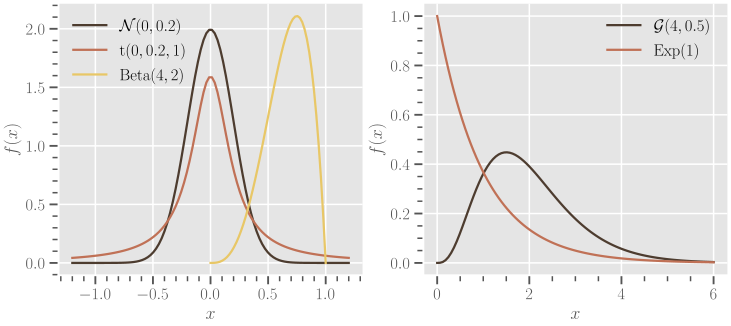
\includegraphics[width=\linewidth]{01_Rozklady_1D}
	\caption{\textbf{Jednowymiarowe zmienne losowe.} Przykładowe gęstości zmiennych losowych z tabeli \ref{tab:przykladowe_zmienne_losowe}.\label{fig:przykladowe_zmienne_losowe}}
\end{figure}

Do opisu zmiennych losowych \emph{wielo}wymiarowych, oprócz gęstości łącznej rozkładu wyróżniamy dodatkowo gęstości warunkowe i brzegowe. Opisują one jak zachowuje się współrzędna wektora losowego, jeśli pozostałe z nich przyjmą pewne wartości, lub jeśli kompletnie wyłączymy ich wpływ.

\begin{df}[Rozkłady brzegowy]
	Rozpatrzmy d-wymiarową zmienną losową $\mathbf{X} = [X_1, X_2, \dots, X_d]$ o gęstości $f(x_1, \dots, x_d)$. Gęstość rozkładu brzegowego $X_j$ definiujemy jako:
	$$f_j(x_j)=\int_{-\infty}^{\infty}\dots\int_{-\infty}^{\infty} f(x_1, \dots, x_{j-1}, x, x_{j+1}, \dots, x_d)  dx_1\dots dx_{j-1} dx_{j+1} \dots dx_d.$$
\end{df}

\begin{df}[Rozkład warunkowy]
	Rozpatrzmy d-wymiarową zmienną losową $\mathbf{X} = [X_1, X_2, \dots, X_d]$ o gęstości $f(x_1, \dots, x_d)$. Gęstość rozkładu warunkowego $X_j \vert X_k$ definiujemy jako:
	$$f_{j|k}(x_j|x_k) = \frac{f(x_1, \dots, x_d)}{f_k(x_k)}.$$
\end{df}


\section{Rozkłady wielowymiarowe}
\label{sec:rozklady_wielowymiarowe}
Naturalnym jest więc, że w praktyce często rozważamy modele wielowymiarowych zmiennych losowych, które mają regularne, łatwe do opisania gęstości łączne. Rozkłady jednowymiarowe z tabeli \ref{tab:przykladowe_zmienne_losowe} w naturalny sposób znajdują swoje rozszerzenia na więcej wymiarów (\cite{MultivariateDistributions}, \cite{Cherubini_Copula_Methods_in_Finance}). Najpopularniejszym tego przykładem jest rodzina $d$-wymiarowych rozkładów eliptycznych, do której należą rozkłady o gęstości postaci:

$$ f_{\mathcal{N}}(x, \mu, \Sigma) = k_d \vert\Sigma\vert^{-0.5}g\big((x-\mu)^T\Sigma^{-1}(x-\mu)\big).$$

W powyższej reprezentacji, $k_d \in\mathbb{R}$ jest stałą zależną od wymiaru, $\mu$ jest $d$-wymiarowym wektorem średnich, $\Sigma \in \mathbb{R}^{d \times d}$ to symetryczna, dodatnio zdefiniowana macierz, a $g \colon [0, \infty) \mapsto [0, \infty)$ jest pewną funkcją która nie zależy od wymiaru wektora.

Dla odpowiednio dobranych $g$ i $k_d$ otrzymamy w tej rodzinie wielowymiarowy rozkład normalny, czy wielowymiarowy rozkład t. Powstają one przy odpowiednio $k_d=(2\pi)^{-0.5d}$ i $g(s) = \exp(-0.5 t)$, lub $k_d=\Gamma(\frac{\nu + d}{2})/\Gamma(\frac{\nu}{2})$ i $g(s) = \big(1 + \frac{t}{\nu})^{-(\nu + d)/2}$.
\begin{figure}[H]
	\centering
	\includegraphics[width=0.45\linewidth]{01_MultivariateGaussian}	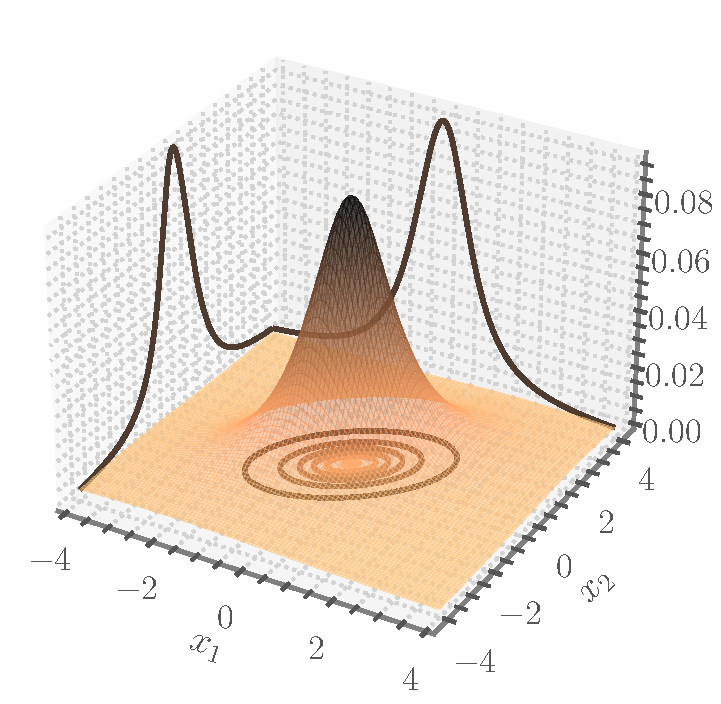
\includegraphics[width=0.45\linewidth]{01_MultivariateStudent}
	\caption{\textbf{Rozkłady eliptyczne.} Gęstości przykładowych rozkładów eliptycznych ($d=2, \mu=[0, 0], \Sigma = \big[\begin{smallmatrix}2&1\\1&2\end{smallmatrix}\big]$). Lewy panel: $2$-wymiarowy rozkład normalny. Prawy panel: $2$-wymiarowy rozkład t ($\nu = 0.5$).\label{fig:multivariate_gaussian_student}}
\end{figure}

Używając rozkładów eliptycznych implikujemy model w którym rozkłady brzegowe pochodzą z tej samej rodziny. Obserwując rysunek \ref{fig:multivariate_gaussian_student}, można rozpoznać charakterystyczne kształty rozkładów brzegowych. Manipulując różnymi rozkładami eliptycznymi możemy więc zamodelować różne struktury korelacji między zmiennymi, czy też ciężkość ogonów, lecz tracimy swobodę wyboru rozkładów brzegowych. \cite{Markovitz_MPT} i jego model bazują właśnie na rozkładzie multinormalnym ponieważ zakładają, że wektor średnich i macierz korelacji wystarczająco opisuje rozkład zwrotów aktywów rynkowych. Podejście to łatwo obalić ze względu na empiryczne dowody ciężkoogonowego charakteru zachowania rynku akcji (\cite{Taleb_BS_is_BS}, \cite{Mandelbrot_NonGaussianity}), czy zjawiska niesymetrycznej, silniejszej korelacji w lewym ogonie (\cite{Taleb_BS_is_BS}, \cite{AssymetricEquityDependency}). Nie mniej jednak nie da się odmówić, że ten prosty model jest wystarczający aby uświadomić jak istotny jest wpływ zależności komponentów na zachowanie całego systemu.\\


\mgrclosechapter